\problemname{Fladdermusen}

Fladdermusen Båtman bor i en stor grotta med många andra fladdermöss.
Båtman har precis fått ett nytt jobb som den officiella fladdermus-brevbäraren.
Detta betyder att Båtman måste leverera brev mellan vissa punkter i grottan.

Grottan är två-dimensionell och rektangulärformad med höjd $H$ och bredd $W$ cm.
Den är också fylld med totalt $N$ stycken \emph{stalagmiter} och
\emph{stalaktiter}.  En \emph{stalagmit} är en vertikal droppstenformation som
växer upp från grottans golv, och en \emph{stalaktit} är en vertikal
droppstenformation som växer ner från grottans tak.
Både stalagmiterna och stalaktiterna i grottan är oändligt tunna, men går inte
att flyga igenom.

Båtman har fått en lista på $Q$ stycken brev som måste levereras.
Varje brev måste hämtas upp från en punkt i grottan och levereras till en
annan punkt. Båtman undrar nu, för varje brev, hur långt hen måste flyga
för att leverera det från startpunkten till ändpunkten, och ber dig om
hjälp för att räkna ut detta.

Fladdermöss (inkluderat Båtman) kan endast flyga rakt upp, rakt ner,
rakt vänster och rakt höger, men kan byta mellan dessa fyra rikntningar
när som helst.\footnote{Läsaren kanske känner igen att vi är intresserade av \emph{Manhattan}-avstånd i det här problemet.}
Båtman kan alltså exempelvis flyga 0.4 cm till höger, och sen byta till att flyga
4.3 cm uppåt.

\begin{figure}[!h]
\begin{center}
  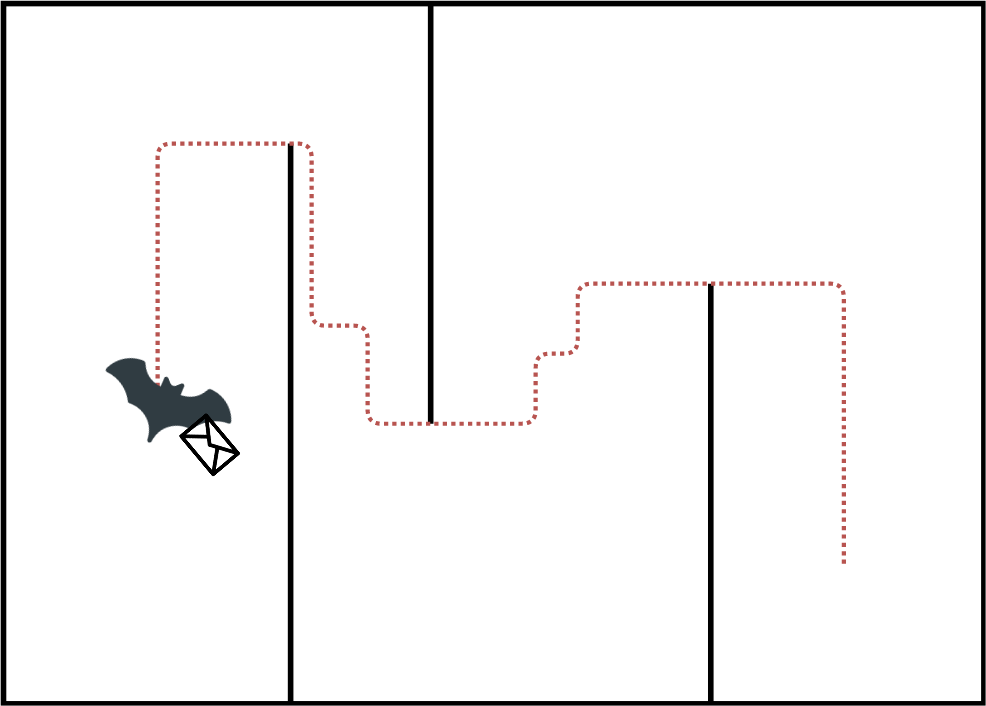
\includegraphics[width=12cm]{fladdermus.png}
\end{center}
  \caption{Illustration av första exempelfallet. Den prickade linjen visar
  en möjlig kortaste flygväg av längd 12 för att leverera det första brevet.}
\end{figure}

\section*{Indata}
Den första raden innehåller fyra heltal $N,Q,H,W$ vilket representerar:
\begin{itemize}
  \item $1 \le N\le 200\,000$ är totala antalet stalagmiter och stalaktiter.
  \item $1 \le Q\le 200\,000$ är antalet brev Båtman som ska levereras.
  \item $1 \le H,W\le 10^9$ är höjden respective bredden på grottan.
\end{itemize}
Därefter kommer $N$ rader som är på någon av följande former:
\begin{itemize}
  \item $1\enspace x\enspace y$, vilket betyder att det finns en stalagmit
    som växer upp från punkten $(x,0)$ till punkten $(x,y)$.
  \item $2\enspace x\enspace y$, vilket betyder att det finns en stalaktit
    som växer ner från punkten $(x,H)$ till punkten $(x,y)$.
\end{itemize}
Ingen stalagmit/stalaktit når hela vägen från taket till botten,
och stalagmiterna/stalaktiterna är all helt inuti grottan,
d.v.s.\ $1\le x_{i} < W$ och $1\le y_{i} < H$.

Därefter kommer $Q$ rader med fyra heltal
$x_{1},y_{1},x_{2},y_{2}$ ($1\le x_{1},x_{2} < W$, $1\le y_{1},y_{2}< H$) vilket representerar att ett brev ska levereras från
punkten $(x_{1},y_{1})$ till punkten $(x_{2},y_{2})$.

\textbf{Det är garanterat att alla $x$-koordinater i indatan är unika.}

\section*{Utdata}
Ditt program ska skriva ut $Q$ rader, ett för varje brev.
Den $i$:e raden ska innehålla ett heltal som är den minsta
sträckan Båtman måste flyga för att leverera det $i$:e brevet.

\section*{Poängsättning}
Din lösning kommer att testas på en mängd testfallsgrupper.
För att få poäng för en grupp så måste du klara alla testfall i gruppen.

\noindent
\begin{tabular}{| l | l | l |}
\hline
Grupp & Poängvärde & Gränser \\ \hline
$1$    & $15$         & $N,Q\le 100$ och $H,W\le 500$ \\ \hline
$2$    & $20$         & $N,Q \le 2000$ och $H,W\le 2\cdot 10^6$\\ \hline
$2$    & $25$         & Det finns max 15 stalaktiter \\ \hline
$3$    & $40$         & Inga ytterligare begränsningar \\ \hline
\end{tabular}
